\documentclass{article}

\usepackage{graphicx}
\usepackage{tikz}
\usepackage{tikzsymbols}
\usetikzlibrary{calc,patterns,shapes.geometric}
\pagestyle{empty}
\usepackage[margin=0pt]{geometry}
\geometry{papersize={14in,12in}}

\def\centerarc[#1](#2)(#3:#4:#5){\draw[#1] ($(#2)+({#5*cos(#3)},{#5*sin(#3)})$) arc (#3:#4:#5);}

\begin{document}
	\begin{figure}
		\centering
		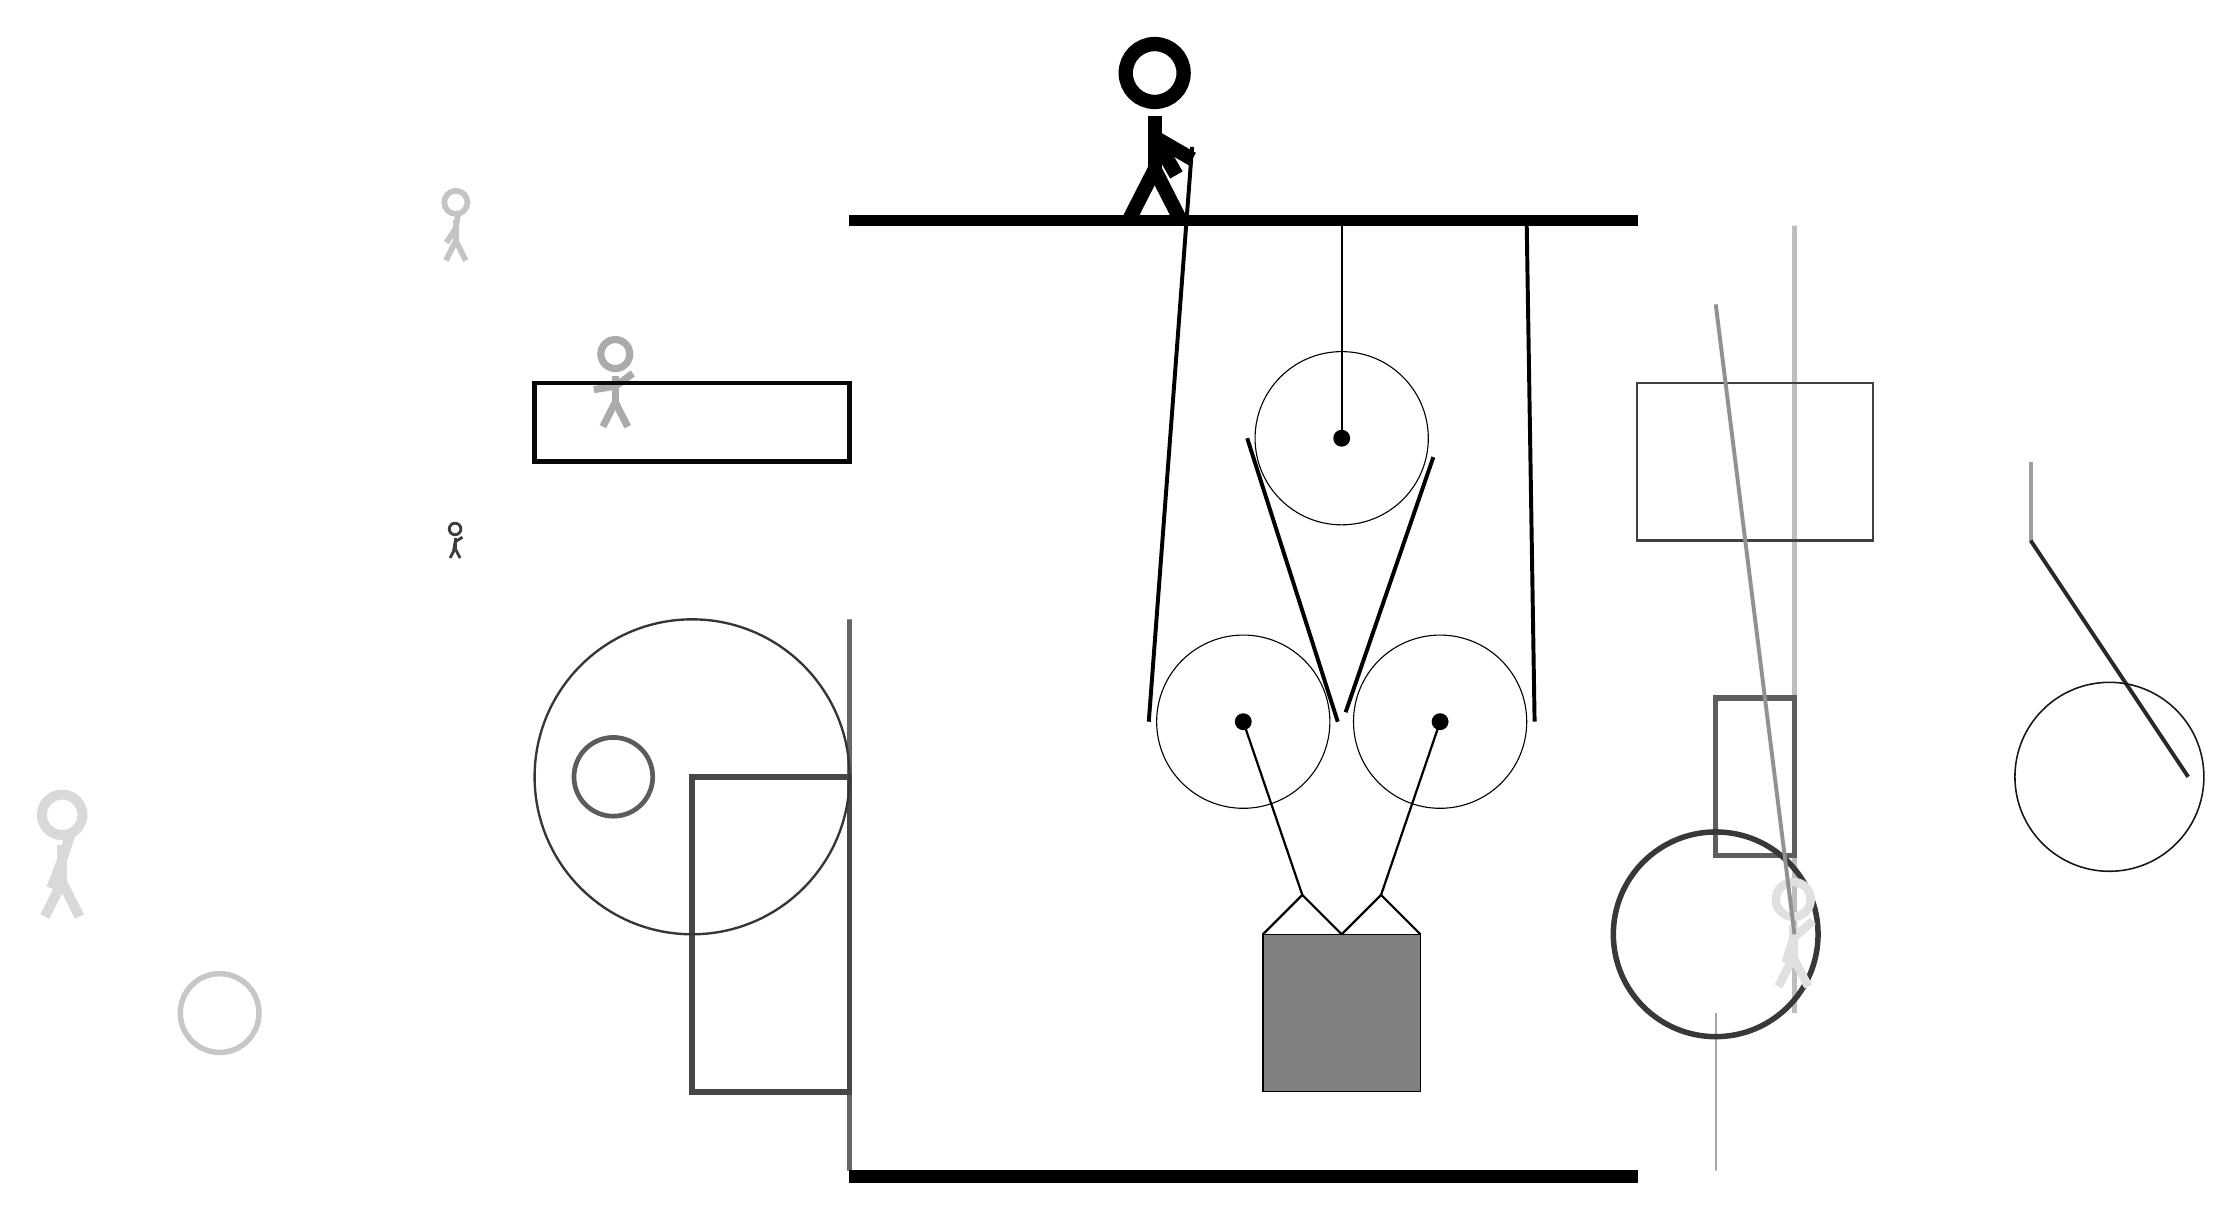
\begin{tikzpicture}
			%%%%% START %%%%%
			
			\draw[fill=black] (-4, 9) rectangle (6, 9.125);
			
			\draw (1, 2.7) circle (1.1);
			\draw[fill=black] (1, 2.7) circle (0.1);
			
			\draw (2.25, 6.3) circle (1.1);
			\draw[fill=black] (2.25, 6.3) circle (0.1);
			\draw[thick] (2.25, 6.3) -- (2.25, 9);
			
			\draw (3.5, 2.7) circle (1.1);
			\draw[fill=black] (3.5, 2.7) circle (0.1);
			
			\draw[thick] (3.5, 2.7) -- (2.75, 0.5);
			\draw[thick] (1, 2.7) -- (1.75, 0.5);
			\draw[thick]  (1.25, 0) -- (1.75, 0.5) -- (2.25, 0);
			\draw[thick]  (2.25, 0) -- (2.75, 0.5) -- (3.25, 0);
			\draw[fill=black!50] (1.25, 0) rectangle (3.25, -2);
			
			\draw[line width=0.5mm] (0.35, 10) --  (-0.2, 2.7);
			\centerarc[line width=0.5mm](1, 2.7)(180:360:1.2000000000000002);
			\draw[line width=0.5mm] (2.2, 2.7) -- (1.05, 6.3);
			\centerarc[line width=0.5mm](2.25, 6.3)(-20:180:1.2000000000000002);
			\draw[line width=0.5mm](3.414, 6.06) -- (2.3, 2.82);
			\centerarc[line width=0.5mm](3.5, 2.7)(160:360:1.2000000000000002);
			\draw[line width=0.5mm](4.7, 2.7) -- (4.6, 9);
			
			\node at (-0.07, 10.2) {\Strichmaxerl[10][120][-30]};
			
			\draw [line width=0.2mm, color=black!51](-9, 9) circle (0.0);
			
			\draw[line width=0.7mm, color=black!60] (-4, 4) rectangle (-4, -3);
			\draw[line width=0.7mm, color=black!72] (-4, 2) rectangle (-6, -2);
			\draw [line width=0.6mm, color=black!64](-7, 2) circle (0.5);
			
			\draw[line width=0.5mm, color=black!38](11, 5) -- (11, 6);
			\node[line width=0.4mm, color=black!33] at (-7, 7) {\Strichmaxerl[5][9][36]};
			\draw[line width=0.7mm, color=black!26] (8, -1) rectangle (8, 9);
			\node[line width=0.7mm, color=black!76] at (-9, 5) {\Strichmaxerl[2][81][32]};
			\node[line width=0.4mm, color=black!23] at (-9, 9) {\Strichmaxerl[4][57][81]};
			\draw[line width=0.3mm, color=black!35] (7, -1) rectangle (7, -3);
			\draw [line width=0.7mm, color=black!22](-12, -1) circle (0.5);
			\draw [line width=0.3mm, color=black!79](-6, 2) circle (2.0);
			\draw[line width=0.7mm, color=black!63] (8, 1) rectangle (7, 3);
			\draw [line width=0.7mm, color=black!78](7, 0) circle (1.3);
			\draw[line width=0.5mm, color=black!84](11, 5) -- (13, 2);
			\node[line width=0.4mm, color=black!15] at (-14, 1) {\Strichmaxerl[7][69][72]};
			
			\draw[line width=0.3mm, color=black!75] (6, 7) rectangle (9, 5);
			
			\node[line width=0.7mm, color=black!12] at (8, 0) {\Strichmaxerl[6][73][41]};
			\draw[line width=0.5mm, color=black!43](8, 0) -- (7, 8);
			\draw [line width=0.2mm, color=black!91](12, 2) circle (1.2);
			\draw[line width=0.6mm, color=black!97] (-4, 6) rectangle (-8, 7);
			
			
			\draw[fill=black] (-4, -3) rectangle (6, -3.15);
			
			%%%%% END %%%%%
		\end{tikzpicture}
	\end{figure}	
\end{document}